% Model 3: inherited states, compound hazards, numerical check and resilience results.
\subsection{Post-Construction Resilience under Compound Disasters}\label{sec:model3}
Task~3 tests the completed belt for 50 years from Model~2's year~15 ($t=0$). Random droughts constrain canal supply, storms remove cover, and Model~1 tracks subsequent growth and recovery.

\subsubsection[Drought Rationing and Storm Damage]{Model construction}
\paragraph{Inherited stands and compound hazards.} The stress test starts from the year-15 cover, soil water and irrigation quotas of cohorts A, B and C (Figure~\ref{fig:m2-plan}a). Disasters enter through two channels \cite{EN14,EN15}. A shared yearly drought switch $D_t^{\mathrm{dr}}$ cuts rain ($\times0.40$), raises demand ($\times1.15$), shrinks canal caps ($\times0.70$) and multiplies the storm rate by $1.5$. Sandstorms, abrasion and burial are represented by a random loss of cover:
\begin{equation}\label{eq:m3-hazard}
N_t\mid D_t^{\mathrm{dr}}\sim\mathrm{Poisson}\big(\lambda_0 e^{\alpha_\lambda t}\gamma^{D_t^{\mathrm{dr}}}\big),\qquad
R_t=\prod_{q=1}^{N_t}(1-U_{t,q}),\quad U_{t,q}\sim\mathrm{U}(0.10,0.50).
\end{equation}
Climate drift slowly raises wind ($e^{\alpha_u t}$, acting through Model~1's $\mathrm{ET}_0$) and lowers rain ($e^{\alpha_R t}$).

\paragraph{One year of the belt.} Canal water is rationed month by month (PV washing first, the rest shared in proportion to requests), the unchanged Model~1 map $\Phi$ grows each cohort, and the storm retention is applied at year end:
\begin{equation}\label{eq:m3-step}
(\widetilde V_{j,t+1},\,M_{j,t+1})=\Phi\big(V_{j,t},M_{j,t};I_{j,t,m}\big),\qquad V_{j,t+1}=R_t\,\widetilde V_{j,t+1}.
\end{equation}
A warning occurs when half the belt is simultaneously below $0.30K$ ($11.4\%$ cover). Resistance is the restricted mean time to first warning, $\mathrm{RMST}(50)=\mathbb E[\min(\tau_{\mathrm{proj}},50)]$, and recovery is the difference between ever-crossed and currently low area. The physical state $(V,M)$ continues after a warning, allowing regrowth.

\subsubsection[Monte Carlo Stress Tests and Markov Verification]{Solution approach}
We simulate $6{,}000$ paths over 50 years for each reference case and $3{,}000$ per sensitivity case. Baseline storm rate is $\lambda_0=0.25$/yr, drought probability is $0.12+0.002t$, and annual wind, rain and storm-rate trends are $+0.5\%$, $-0.5\%$ and $+1\%$. These are declared stress scenarios, not calibrated forecasts. Tests vary storm rate and loss on a $3\times3$ grid, remove drought, its storm multiplier or climate drift, and compare warning levels $0.20K$ and $0.40K$.

An independent stationary Markov calculation groups stands by cover and stored water. Figure~\ref{fig:m3-check} compares its first-warning probabilities with Monte Carlo 95\% intervals at years 10, 30 and 50. Recovery and project-level outcomes come from the continuing non-stationary simulation.

\begin{figure}[!htbp]
  \centering
  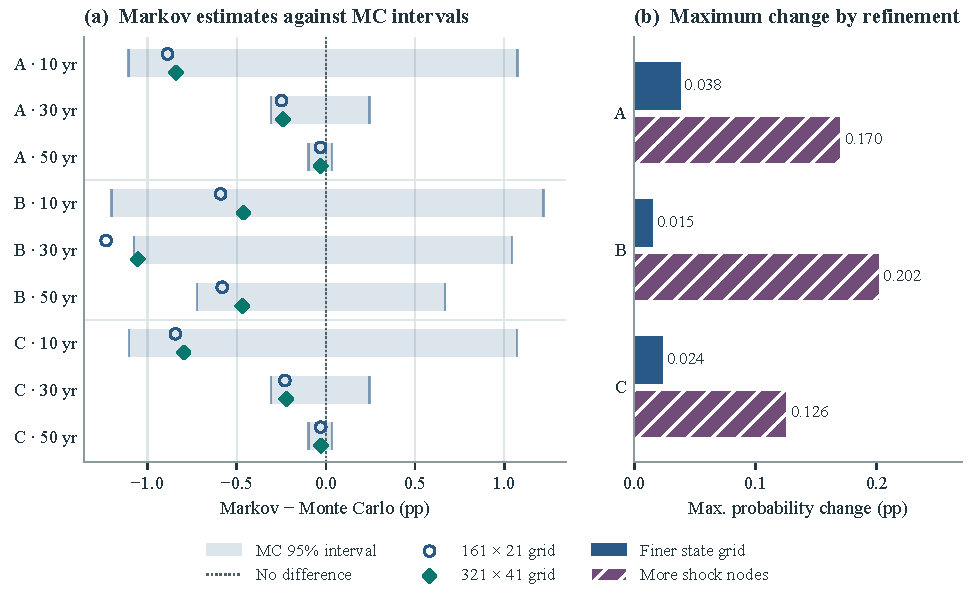
\includegraphics[width=\linewidth]{../Figures/Paper2026_Polished/fig14_markov_validation.pdf}
  \caption{Stationary Markov validation and refinement sensitivity.}
  \label{fig:m3-check}
\end{figure}

\subsubsection[Warning Risk, Vegetation Recovery, and Water Limits]{Results}
\paragraph{Early warnings and partial recovery.} In the baseline simulation, $77.5\%$ of paths trigger a belt warning by year~10, and all $6{,}000$ paths do so by year~50. The 50-year restricted mean time to first warning is $7.1$\,yr for the belt and $16.1$\,yr for core strip B (Figure~\ref{fig:m3-res}a). By year~50, almost all $300$\,ha has crossed the threshold at some point. About $99$\,ha has returned above the threshold and $200$\,ha is still below it (Figure~\ref{fig:m3-res}b). Cumulative benefit is $4{,}762\text{ effective ha}\cdot\text{yr}$, or $65.5\%$ of the climate-drift-only case (Figure~\ref{fig:m3-res}d).

\begin{figure}[!htbp]
  \centering
  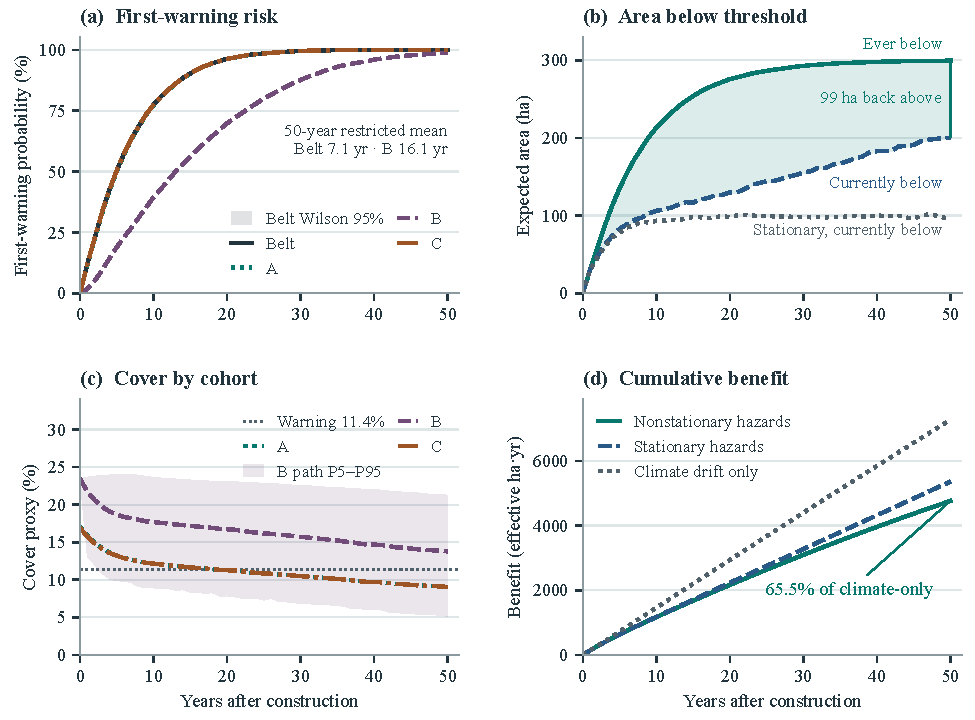
\includegraphics[width=\linewidth]{../Figures/Paper2026_Polished/fig15_resilience.pdf}
  \caption{First-warning risk, recovery and cumulative ecological benefit.}
  \label{fig:m3-res}
\end{figure}

\paragraph{Risk drivers and verification.} $\mathrm{RMST}(50)$ ranges from $41.8$\,yr for rare, mild storms to $2.8$\,yr for frequent, severe storms (Figure~\ref{fig:m3-sens}a). Requesting $20\%$ more water raises the baseline value from $7.1$ to $8.1$\,yr (panel b). In May of the first post-construction drought year, both plans receive the same $126{,}000$\,m$^3$ of ecological water at the delivery limit (panel c, rounded). That is about $26\%$ below normal May delivery under the baseline request. In the stationary check, all nine fine-grid estimates lie within the Monte Carlo $95\%$ intervals (Figure~\ref{fig:m3-check}). Refining the state grid and storm quadrature changes probabilities by at most $0.04$ and $0.20$ percentage points, respectively.

\paragraph{Summary.} Some stands regain cover after a warning. In the tested scenarios, the dry-season capacity to deliver water limits the value of raising the annual request.

In Figure~\ref{fig:m3-res}, bands show 95\% Wilson intervals for belt risk and 5th--95th path percentiles for cohort B cover. In Figure~\ref{fig:m3-sens}, the 30\% mean-loss grid column uses $[0.15,0.45]$ for loss per storm, versus $[0.10,0.50]$ in the baseline.

% Finish the preceding floats before placing this exhibit and the overall assessment.
\clearpage
\begin{figure}[H]
  \centering
  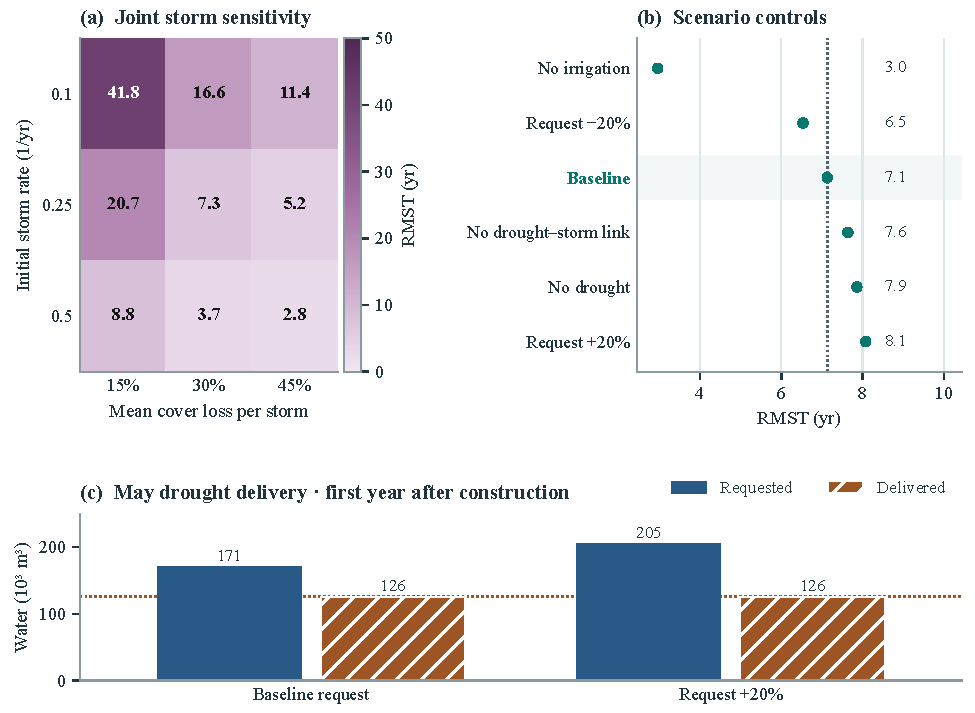
\includegraphics[width=\linewidth]{../Figures/Paper2026_Polished/fig16_storm_and_delivery.pdf}
  \caption{Storm sensitivity and May irrigation delivery under drought.}
  \label{fig:m3-sens}
\end{figure}
